\renewcommand{\proofname}{Доведення}
\renewcommand{\chaptername}{РОЗДІЛ}
\chapter{Тренди серед мобільних фреймворків}
\label{ch1}

\section{Розробка крос-платформних мобільних додатків}
\label{section.1.1}
Завдяки міжплатформенній розробці підприємства та організації змогли охопити ширшу аудиторію, ефективніше та з меншими витратами.
React Native був представлений Facebook у 2015 році.
React Native - це фреймворк для мобільних додатків з відкритим кодом, який використовує React із власними можливостями платформи для розробки додатків для Android, iOS, Web та UWP.

Серед рішень, що використовують React Native: Facebook, Instagram, Tesla, Uber Eats, Discord, Wix, Walmart.

Flutter був представлений Google у травні 2017 року. Але випуск стабільної версії відбувся у грудні 2018 року.
Flutter також має відкритий вихідний код і використовується для розробки програм для Android, iOS, Linux, Mac, Windows, Google Fuchsia та веб.

Деякі програми, створені за допомогою Flutter, це: Google Ads, Alibaba.com, Realtor.com.

Оскільки Flutter та React-Native стали найгарячішою темою останніх днів та конкурентними дебатами серед спільноти розробників, багато розробників залижаються у невизначеності, визначаючи, яку платформу вибрати.

\section{Тренди}\label{section.1.2}

\begin{figure}
    \label{fig:flutter_react_trend_5_years}
    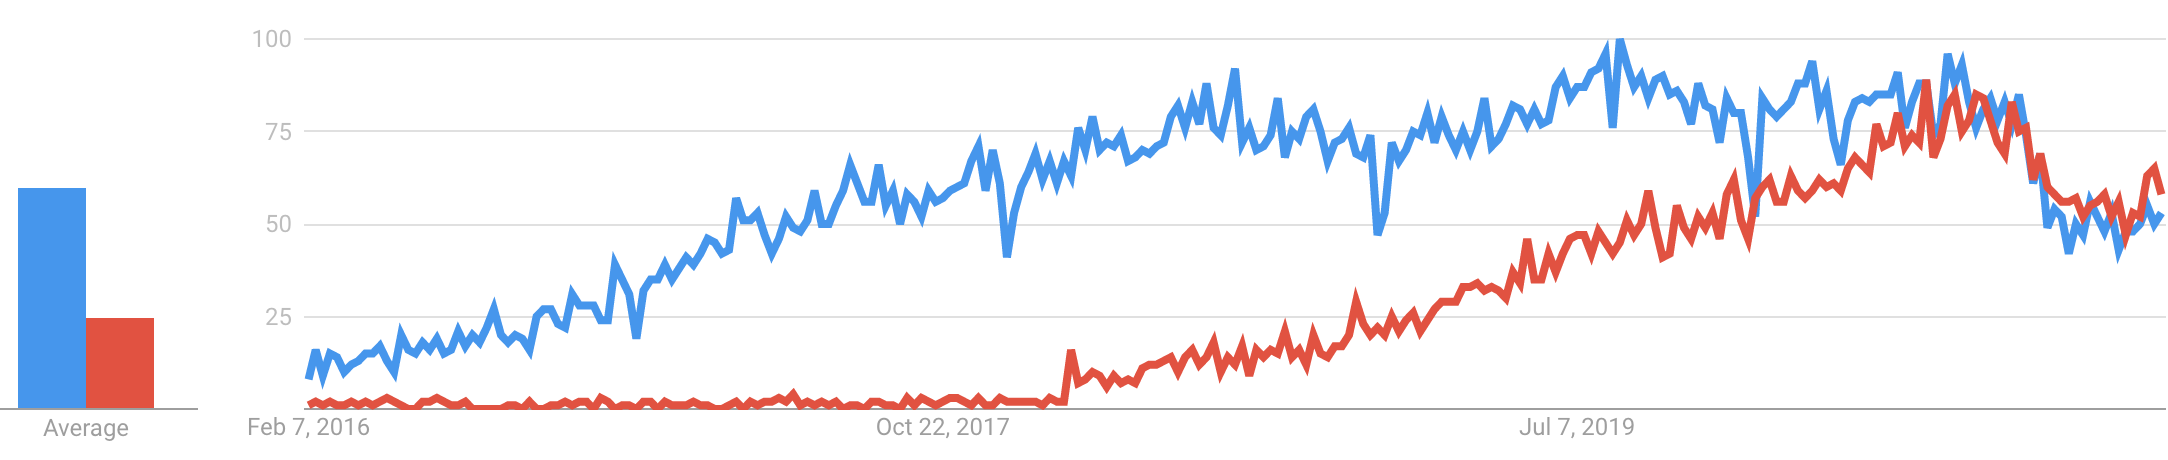
\includegraphics[scale=0.4]{flutter_react_trend_5_years.png}

    Відповідно до Google Trends за 5 років
\end{figure}

На Google Trends за останні п’ять років Flutter випередив React Native.
Але це не визначає, що Flutter - кращий варіант, ніж React Native.

Що стосується міжплатформенних тенденцій розвитку технологій мобільних додатків, то і React Native, і Flutter досить схожі за популярністю, і обидва вони все ще досить молоді (React Native вийшов у 2015 році, Flutter у 2017 році).
Обидві технології посідають дуже високе місце на GitHub із 112 тис. зірок (Flutter) \cite{flutter_gihtub} та 93.2 тис. (React Native) \cite{rn_gihtub} за лютий 2021.

Ми бачимо, що інтерес до Флаттера значно зріс у 2021 році і швидко зростає.

\section{Переваги Flutter}\label{section.1.3}
\begin{enumerate}
    \begin{item}
        Одна кодова база.
        Flutter підтримує як мобільні платформи Android, так і iOS, і оскільки він відображає все самостійно, він дозволяє запускати все з однієї кодової бази.
        Це велика економія часу!
    \end{item}
    \begin{item}
        Красиві інтерфейси в найкоротші терміни.
        У Flutter користувальницький інтерфейс побудований за допомогою віджетів, невеликих будівельних блоків інтерфейсу, зібраних за допомогою техніки, що називається Композиція.
        Весь процес схожий на використання компонентів React.
        Існує два набори віджетів, що доступні нестандартно: Material Design, який сумісний з дизайнерськими вказівками Google, та Cupertino, сумісний з Apple's Interface Guidelines для iOS .
    \end{item}
    \begin{item}
        Візуалізація пікселів.
        Flutter управляє кожним пікселем екрану, тому ми можемо бути впевнені, що наші віджети будуть виглядати однаково на кожному мобільному пристрої (навіть на старих), по суті усуваючи наші потенційні проблеми з підтримкою пристрою.
        Це, в свою чергу, дозволяє нам створювати дивовижні на вигляд користувальницькі інтерфейси, які виглядають абсолютно однаково як на Android, так і на iOS з єдиною кодовою базою.
    \end{item}
    \begin{item}
        Швидша розробка за допомогою Hot reload.
        Тут Flutter справді сяє: функція гарячого перезавантаження забезпечує можливість внесення змін на льоту, дозволяючи побачити їх відразу під час розробки.
        Ця функція значно покращує процес розробки додатків!
    \end{item}
    \begin{item}
        Розробка міжплатформенних додатків.
        Як уже зазначалося, Flutter SDK - це міжплатформенний інструмент, який дозволяє нам розробляти для настільних ПК, мобільних пристроїв та Інтернету за допомогою єдиної кодової бази.
        Це також дозволяє створювати чудові виразні інтерфейси за допомогою віджетів, шарів та інтерактивних активів Flutter.
    \end{item}
\end{enumerate}

\begin{figure}
    \label{fig:stackoverflow_survey_2020}
    \begin{center}
        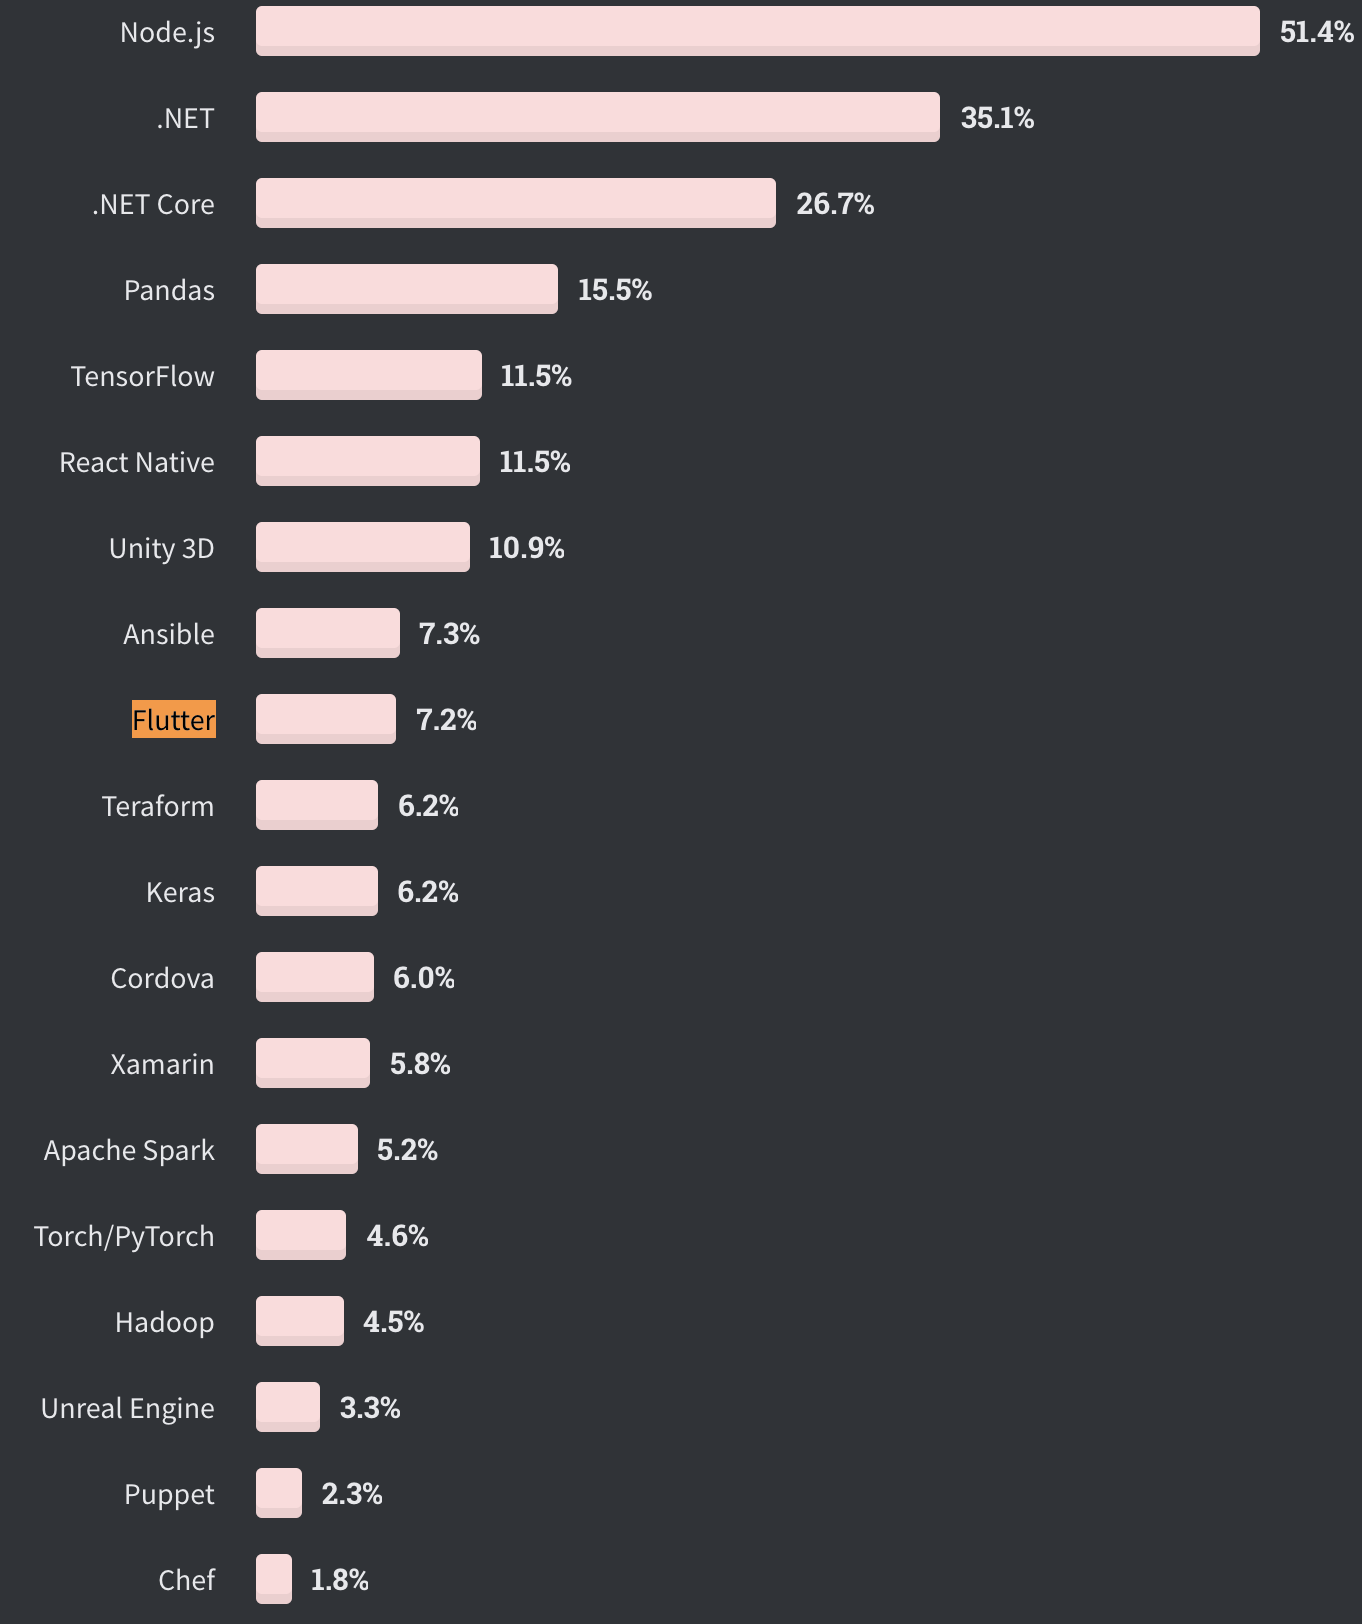
\includegraphics[scale=0.4]{stackoverflow_survey_2020.png}
    \end{center}

    Основна популярність за результатами опитування, яке охопило 40 000 відповідей.
    \cite{stackoverflow_survey_2020}
\end{figure}

\section{Недоліки Flutter}\label{section.1.4}
\begin{enumerate}
    \begin{item}
        Він має обмеження щодо надання інтерфейсу користувача на власних платформах, наприклад, відео на Apple TV або Android TV.
    \end{item}
    \begin{item}
        Функції, що нещодавно додані в рідних системах iOS та Android, природно будуть представлені у Flutter пізніше, ніж у їхніх рідних версіях.
    \end{item}
    \begin{item}
        Незважаючи на те, що Flutter легко вивчити, вам, мабуть, знадобиться певний досвід розробки власних додатків, щоб створити функціональний крос-платформний додаток.
    \end{item}
\end{enumerate}

\section{Переваги React Native}\label{section.1.5}
\begin{enumerate}
    \begin{item}
        Це зрілий фреймворк зі стабільним API, який підтримується Facebook.
    \end{item}
    \begin{item}
        Легко навчитися розробникам React та JavaScript.
        Ви можете скористатися наявними бібліотеками React, інструментами, фреймворками та навчальними посібниками.
        Структура також має велику спільноту розробників.
    \end{item}
    \begin{item}
        Так само, як Flutter, він дозволяє швидко розроблювати додатки iOS, Android та Web зі спільною кодовою базою.
    \end{item}
    \begin{item}
        React Native дозволяє додавати новий код до запущеної програми, що зменшує ризик втрати деяких функціональних можливостей під час повного перезавантаження або відновлення програми.
    \end{item}
\end{enumerate}

\section{Недоліки React Native}\label{section.1.6}
\begin{enumerate}
    \begin{item}
        У ньому все ще бракує певних спеціальних модулів, специфічних для платформи, і для їх створення вам може знадобитися досвід native розробника.
    \end{item}
    \begin{item}
        Навігація не є плавною.
    \end{item}
    \begin{item}
        Міжплатформна розробка може спричинити проблеми з продуктивністю оскільки використовується додатковий рівень інтерпретації коду в runtime середовищі.
    \end{item}
    \begin{item}
        Це не найкращий вибір для програм, які потребують складну анімацію (на приклад ігри).
    \end{item}
\end{enumerate}

\section{Мови програмування}\label{section.1.7}

Flutter використовує мову, що називається Dart.
Це мова, яка має синтаксис, подібний до Java та Javascript.

Простим прикладом коду в Dart буде:
\begin{lstlisting}[style=light, language=Python,label={lst:vectorimg},caption=Dart Hello World]
void main () { 
  print ("Hello World!"); 
}
\end{lstlisting}

React Native використовує Javascript.
React Native побудований поверх React, який побудований на Javascript.
Тому, якщо вам доведеться вивчити React Native, вам знадобляться попередні знання Javascript.

Javascript існує довкола спільноти розробників програмного забезпечення дуже давно, і існує безліч ресурсів, на яких можна навчитися javascript.
Простим прикладом коду в javascript буде:

\begin{lstlisting}[style=light, language=Python,label={lst:vectorimg},caption=Dart Hello World]
  alert("Hello World!");
\end{lstlisting}

\section{Спільнота}\label{section.1.8}

Flutter і Dart були представлені спільноті розробників нещодавно, і порівняно, у неї менша спільнота розробників.
Google витратив багато на розробку Dart, і спільнота продовжує зростати.
Flutter має спільноти на StackOverflow, Slack та багатьох інших платформах.

React Native має більшу спільноту розробників, ніж Flutter, сприяючи його розвитку.
Спільнота Javascript є навіть більшою, ніж спільнота React Native, оскільки вона існує вже дуже давно, і допомогу можна знайти майже скрізь в Інтернеті.
Це, безумовно, пояснює, чому React Native має вищий рівень прийняття в порівнянні з Flutter.
Крім того, підтримка React, React Native та Javascript в Інтернеті є більш доступною.
Є мільйони рядків коду, які є у вільному доступі в Інтернеті, і їх можна просто «зняти» та використовувати у своїх проектах.
На сторінці спільноти React Native на їх офіційному веб-сайті вказані інші платформи, що вміщують їхні спільноти, такі як StackOverflow та Medium.

\section{Віджети інтерфейсу користувача}\label{section.1.9}
Найкраще у Dart - це те, що він постачається з повним набором віджетів інтерфейсу, які можна підняти прямо з коробки та використовувати.
В React Native, набір віджетів інтерфейсу мінімальний, і тому розробникам програмного забезпечення та програмістам доводиться звертатися до сторонніх бібліотек для віджетів інтерфейсу, і іноді їм доведеться створювати власні віджети інтерфейсу.

\section{Flutter vs React Native - хто переможець?}\label{section.1.10}
Ми вже висвітлювали основні характеристики Flutter і те, чим він відрізняється від своїх інших крос-платформних систем, тому залишається останнє питання: чи насправді це майбутнє розвитку мобільних пристроїв?
Чи перемагає він у гонці React Native vs Flutter? Так .

Хоча обидва фреймворки дійсно чудово підходять для розробки мобільних додатків, Flutter пропонує безліч функцій, які можуть допомогти нам розробляти красиві мобільні додатки з кращим користувацьким досвідом і робити це швидше - дозволяючи заощадити більше часу та грошей.
Flutter вже зарекомендував себе у світі розробки мобільних додатків, і я думаю, що 2021 рік - ідеальний час, щоб нарешті спробувати, якщо ви розглядаєте його для свого наступного мобільного MVP.
